% Week 2 排版练习；使用 XeLaTeX + BibTeX。
% 本例不代表真实数据分析，也不是比赛官方提交模板。
% 在仓库根目录：
\documentclass[11pt,letterpaper]{article}
\usepackage[margin=1in]{geometry}
\usepackage{amsmath,amssymb}
\usepackage{booktabs}
\usepackage{graphicx}
\usepackage{pgfplots}
\pgfplotsset{compat=1.18}
\usepackage[numbers,sort&compress]{natbib}
\usepackage{xurl}
\usepackage[colorlinks=true,linkcolor=blue,citecolor=blue,urlcolor=blue]{hyperref}

\title{Week 2: Paper Writing Practice}
\author{MCM Preparation}
\date{}

\begin{document}
\maketitle

\begin{abstract}
This practice document connects a simple question, an assumption, a model,
and its results. We ask how far an object travels at a constant speed of
2 metres per second. Using a constant-speed model, we obtain distances of
10, 20, and 30 metres after 5, 10, and 15 seconds. A table and a figure
present the same calculated values. The model applies only when the speed
remains constant. All values are illustrative; this is a typesetting
exercise rather than a report of measured data.
\end{abstract}

\section{Introduction}
The reading exercise for this week uses a 2023 MCM paper by
Team 2314151~\citep{wordle2023}. The example in this document uses a
separate, elementary motion problem to practise document structure.
Our question is: how far does an object travel in a specified time
when its speed is constant?
We examine how the summary connects to the reported
results in the Wordle paper~\citep{wordle2023}.

\section{Assumptions}
\begin{enumerate}
  \item The object moves along a straight path in one direction.
  \item Its speed remains constant during the interval considered.
  \item Distance and elapsed time are both zero at the starting point.
\end{enumerate}
These assumptions let us use a single speed parameter. Acceleration and
stops are outside the scope of this example.

\section{Notation}
\begin{center}
\begin{tabular}{lll}
\toprule
Symbol & Meaning & Unit \\
\midrule
$t$ & Elapsed time & s \\
$v$ & Constant speed & m/s \\
$s(t)$ & Distance travelled by time $t$ & m \\
\bottomrule
\end{tabular}
\end{center}

\newpage
\section{Model and Solution}
Under the stated assumptions, distance equals speed multiplied by time:
% equation 自动编号；label 给公式起一个稳定的名字。
\begin{equation}
  v = 2\,\mathrm{m/s}.
  \label{eq:speed}
\end{equation}
\begin{equation}
  s(t)=vt, \qquad t\geq 0.
  \label{eq:distance}
\end{equation}
The speed in Equation~\eqref{eq:speed}
is used in Equation~\eqref{eq:distance}.
Here $v=2$ m/s is an illustrative input. Substituting $t=10$ s into
Equation~\eqref{eq:distance} gives $s(10)=20$ m. Each result therefore
has a stated input, a calculation, and a unit.

\section{Results}
% 表格标题在上；label 紧跟 caption。
\begin{table}[htbp]
  \centering
  \caption{Calculated distances for the illustrative constant-speed model.}
  \label{tab:distance}
  \begin{tabular}{rr}
    \toprule
    Time $t$ (s) & Distance $s(t)$ (m) \\
    \midrule
    5 & 10 \\
    10 & 20 \\
    15 & 30 \\
    \bottomrule
  \end{tabular}
\end{table}


% figure 内也可以用 includegraphics 插入队友导出的图片。
\begin{figure}[htbp]
  \centering
  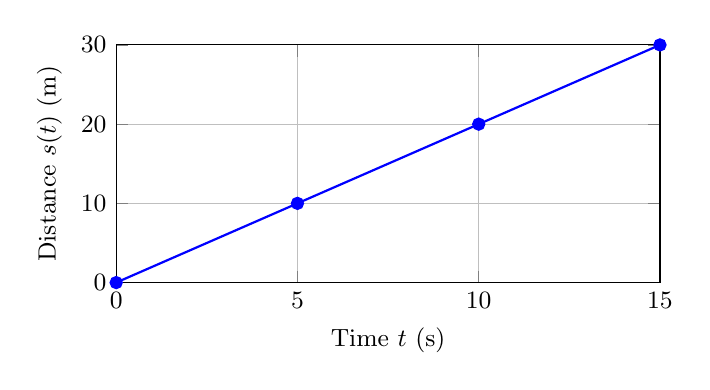
\begin{tikzpicture}
    \begin{axis}[
      width=0.70\textwidth,height=4.6cm,
      xlabel={Time $t$ (s)},ylabel={Distance $s(t)$ (m)},
      xmin=0,xmax=15,ymin=0,ymax=30,
      xtick={0,5,10,15},ytick={0,10,20,30},
      grid=major,
      tick label style={font=\small},
      label style={font=\small}
    ]
      \addplot[blue,thick,mark=*] coordinates {(0,0) (5,10) (10,20) (15,30)};
    \end{axis}
  \end{tikzpicture}
  \caption{Distance increases linearly with time in the illustrative model.}
  \label{fig:distance}
\end{figure}

Table~\ref{tab:distance} lists three calculated values, and
Figure~\ref{fig:distance} shows their common linear trend.
At 10 seconds, the calculated distance is 20 metres. These values follow
from the assumptions; they do not validate the model against observations.

Table~\ref{tab:distance} shows that the distance is 20 m
at 10 s.

Figure~\ref{fig:distance} shows that the distance increases linearly with time.
\clearpage

\section{Sensitivity and Model Evaluation}
For a fixed time $t>0$, Equation~\eqref{eq:distance} implies that a
10\% increase in speed produces a 10\% increase in calculated distance.
This describes the response to one parameter under the same assumptions.

The model is easy to interpret, and its units are consistent. Its main
limitation is that changes in speed are ignored. A real application would
need observations to assess whether the constant-speed assumption is
appropriate and to measure prediction error.

\section{Conclusion}
With an illustrative speed of 2 m/s, the model gives a distance of
20 m after 10 s. The result answers the original question only under the
constant-speed assumption. In a modelling paper, the abstract, model,
tables, figures, and conclusion should tell this same story.

% citep 的文献键来自 references.bib。latexmk 会按需调用 BibTeX。
\bibliographystyle{plainnat}
\bibliography{references}

\end{document}
